\chapter{Methods and Materials}
\label{chapter:mam}

This chapter explains the necessary fundamentals of deep learning to familiarize the reader with the methods used throughout this work. More specifically, \Cref{section:ann} provides an explanatory overlook of the fundamental concepts of feedforward neural networks. Section \ref{section:cnn} touches on the fundamental concepts used by \ac{CNN}s, as well as describe state-of-the-art pre-trained model architectures used throughout this work. The \Cref{section:mam_transfer_learning} explores the concept of repurposing pre-trained models from \ac{CNN} architectures trained on generic datasets. Section \ref{section:overfitting_underfitting} explores a common problem for machine learning algorithms in the context of deep learning, namely, the bias-variance tradeoff and ways to deal with such a problem. Afterward, \Cref{section:ensemble_learning} presents different ways to improve a model's performance through ensemble learning. Next, \Cref{section:metrics} introduces the reader to commonly used metrics to assess performance of a deep learning model. Finally, \Cref{section:out_of_distribution} describes techniques to deal with the detection of out of the training distribution samples, which will be one of the focus points of this work. 

\section{Artificial Neural Networks}
\label{section:ann}
    Artificial Neural Networks compose a category of machine learning algorithms that are inspired by biological neural networks. These structures are comprised of multiple layers, each composed by multiple neurons that can be interpreted as a function described by parameters. \par
    
    Within a neuron, each input $x$ is multiplied by a learnable matrix of weights $w$, where each weight can be seen as the synaptic strength between two neurons. A second parameter is also taken into consideration called bias $b$ that is added to the element wise multiplication between the weights and inputs matrices. With this two parameters a neuron will output a signal (also called activation) according to a activation function $g$ which introduces non-linearity. Mathematically speaking, the output of a neuron can be expressed as:
    \begin{equation}
        f(x)=g(\sum_{i}^{n} x_i w_i + b)
        \label{eqs:neuron}
    \end{equation}
    
    One can look at the process of training an \ac{ANN} as an iterative process that tries to optimize parameters in order to minimize a cost function. There are many different topologies of \ac{ANN}s. One of the most common is the fully connected neural network, where each neuron is connected to every other neuron in the previous layer (see an example in \autoref{fig:fcnn}). \par
    
    \begin{figure}[ht]
      \centering
        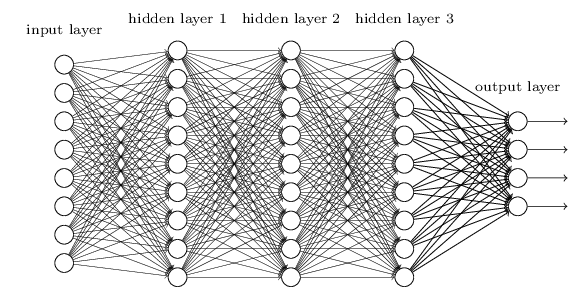
\includegraphics[width=0.8\linewidth]{figs/Deep_Learning.png}
      \caption{Example of a feedforward fully-connected artificial neural network taken from Michael Nielsen \cite{Nielsen2017a}.}
      \label{fig:fcnn}
    \end{figure}

    According to the universal approximation theorem, feedforward \ac{ANN}s, a type of \ac{ANN} where connections between the nodes do not form a cycle, can approximate any function with just one layer. However, for complex functions an increased hidden layer width may be required, which can ultimately be inefficient \cite{Cybenko1989}. Therefore, networks with more hidden layers and with an organization that allows them to create levels of abstraction are often used to solve more complex problems. Such network topologies are called deep neural networks and are part of the broader field of deep learning. There are other deep learning topologies such as deep belief networks, recurrent neural networks, or convolutional neural networks. \par
    
    \subsection{Activation Functions}
    The activation function of a neuron defines the output (activation) of that neuron given an input $z=\sum_{i}^{n} x_i w_i + b$. In this context, several activation functions $g$ have been proposed for \ac{ANN}s, namely:
    \begin{itemize}
        \item The sigmoid function $g(z) = (\frac{1}{1+exp^{-z}})$. Provides smooth gradient between 0 and 1 values, but suffers from computation issues like the vanishing gradients problem;
        
        \item The tanh function $g(z) = (\frac{e^z - e^{-z}}{e^z + e^{-z}}) $. Like the sigmoid except that output values range from -1 to 1, meaning its center is at 0;
        
        \item The ReLU function $g(z) = max(0, z)$. A network with such neurons is able to overcome numerical computation issues like the exploding and vanishing of gradients (typically associated with activation functions like the sigmoid function). Some authors also report that it allows faster convergence in comparison with other activation functions like tanh \cite{alexnet};
        
        \item The softmax function $g(z_i) = \frac{exp(z_i)}{\sum_{i}^{} exp(z_j)}$. It is typically used in the output layer for neural networks which classifies inputs into multiple classes. It normalizes the outputs for each class between 0 and 1, and divides by their sum, giving the probability of the input value being in a specific class \cite{Goodfellow-et-al-2016}.
    \end{itemize}
    
    \subsection{Optimization Algorithms}
    Optimization refers to the process of tuning the parameters of a network in order to improve a specific performance metric (\textit{e.g.}, accuracy). The ideal approach of an optimization algorithm would be to find the global minimum of the cost function, but such an approach is not efficient because it would require testing every possible combination of parameters. Rather, an approximate combination of optimal parameters is often satisfiable, which in turn results in a local minimum of the cost function. Currently, stochastic gradient descent with and without momentum, RMSProp, and Adam belong to the most popular optimization strategies used for deep learning based models \cite{Goodfellow-et-al-2016}. \par
    
    Gradient descent is an algorithm that updates the parameters of a function in the direction in which it decreases most rapidly. Let there be a function $f$ to be minimized, and a vector of parameters $w$ with $n$ elements. One can mathematically look at gradient descent as:
    \begin{equation}
        w_{t+1}=w_t -\eta \nabla f(w_t)
        \label{eq:gradient_update}
    \end{equation}
    where the expression $-\eta \nabla f(w_t)$ can be seen as the step in the parameter space to take at iteration $t$, $\eta$ is the learning rate that controls the magnitude of the update, and the expression $\nabla f(w_t)$ is the vector of first partial derivatives:
    \begin{equation}
        \nabla f(w_t) = (\frac{\delta f(w_t)}{\delta f(w_{t,1})},...,\frac{\delta f(w_t)}{\delta f(w_{t,n})})
        \label{eq:first_derivative}
    \end{equation}
    
    However computing $\nabla f(w_t)$ requires calculating gradients over the whole data which is computationally expensive. Alternatively, in mini-batch gradient descent, the gradient is estimated over a mini-batch (a small number of randomly selected samples from the original dataset), which in theory approximates the true gradient. Mathematically speaking, the true gradient $\nabla f$ calculated over $m$ samples can be approximated by simply calculating the gradient over a mini-batch of $m'$ samples:
    
    \begin{equation}
        \nabla f \approx \frac{\sum_{i=1}^{m'} \nabla f_i}{m'} \approx \frac{\sum_{i=1}^m \nabla f_{i}}{m}
        \label{eq:mini_batch_gradient}
    \end{equation}
    
    A variation of this method adds momentum to the movement of the gradient and is called stochastic gradient descent with momentum \cite{momentum}. This method is analogous to a ball moving on a surface with multiple valleys, accelerating on steep slides and decelerating when it reaches a valley. The intuition behind this method is to add inertia to the gradient descent so that it smooths the overall trajectory, in order to eventually find better convergence points. Mathematically, it can be described as:
    
    \begin{equation}
        \begin{split}
            v_0 = 0\\
            v_{t+1} = -\beta v_t + \eta \nabla f(w_t)\\
            w_{t+1} = w_t - v_{t+1}
        \end{split}
        \label{eq:sgd_momentum}
    \end{equation}  
    where the parameter $\eta$ (learning rate) defines the impact of the current gradient and $\beta$ defines the impact of the previous gradients.
    
    Deep neural networks often have to solve optimization problems with large amounts of dimensions, which poses the question of whether or not it makes sense to use the same learning rate for each of those dimensions, as each one might have different sensitivities. Taking this into consideration, optimization algorithms such as AdaGrad \cite{adagrad} adjusts the learning rate of each parameter individually:
    
    \begin{equation}
        w_{t+1} = w_t - \eta G^{-\frac{1}{2}}_t g_t
        \label{eq:ada_grad}
    \end{equation}  
    where $g_t = \nabla f(w_t)$, $G_t=\sum_{i=1}^{t}g_i g_i^T$ and $\eta$ is the global learning rate.
    
    However, the Adagrad optimization algorithm instigates a decrease in the learning rate which is caused by the accumulation of all past gradients in the denominator. This means that at a certain point in the training procedure, the model becomes unable to learn. RMSProp solves this issue by letting the sum of the accumulated gradients decay (see expressions in \ref{eq:rms_prop}). Therefore, the gradient accumulation is an exponentially weighted moving average of the squared gradients.
    \begin{equation}
        \centering
        \begin{split}
            R[g^2]_t = \rho R[g^2]_{t-1} + (1-\rho)g_t^2\\
            w_{t+1} = w_t - \eta * \frac{g_t}{\sqrt{R[g^2]_t}} 
        \end{split}
        \label{eq:rms_prop}
    \end{equation}  
    where $g_t = \nabla f(w_t)$, the $R[g^2]_t$ is the the running average at time step $t$ (at $t=0$, the $R[g^2]$ is 0), $\rho$ denotes the weight given to the current iteration’s gradient in relation to the past history and $\eta$ is the global learning rate.
    
    Finally, Adam \cite{adam} can be looked at as a combination of RMSprop and stochastic gradient descent with momentum. It uses the squared gradients to scale the learning rate like RMSprop and it takes advantage of momentum by using the moving average of the gradient. The expressions in \ref{eq:adam} describe the weight updates, where $S_t$ is the first-order moment (the mean) and $R_t$ is the second-order moment (the uncentered variance) of the gradients. 
    
    \begin{equation}
        \centering
        \begin{split}
            S_t = \rho_1 S_{t-1} + (1-\rho_1)g_t, S_t = \frac{\hat{S}_t}{1-\rho^t_1}\\
            R_t = \rho_2 R_{t-1} + (1-\rho_2)g_t, R_t = \frac{\hat{R}_t}{1-\rho^t_2}\\
            w_{t+1} = w_t - \frac{\eta}{\sqrt{\hat{R}_t}} \hat{S}_t  
        \end{split}
        \label{eq:adam}
    \end{equation}  
    where $\rho_1$ and $\rho_2$ denotes the weight given to the current iteration’s gradient in relation to the past history and $\rho_1^t$, $\rho_2^t$ are used to correct the initializations of $R_t$ and $S_t$, respectively. Furthermore, $\eta$ is the global learning rate. \par
    
    Despite the popularity of adaptive optimization algorithms like Adam, the choice of the optimization algorithm to be used to train deep neural networks is typically based on the familiarity of the user with it, rather than some analytical judgement \cite{Goodfellow-et-al-2016}. \par 
    
    \subsection{Initialization Strategies}
    The simplest approach to initialize the weights of the network is by setting them to zero. However, by initializing every weight to zero, every neuron will have the same activations, all the calculated gradients will be the same, and consequently, each parameter will suffer the same update. Therefore, it is crucial that the initialization of the weights breaks the symmetry between different units. Drawing from a random Gaussian distribution with mean 0 and deviation 1 would break such symmetry but would also mean that some parameters would have much higher values than others, which would eventually lead to problems like the vanishing or exploding gradients problem. Therefore, different strategies have been proposed to define the distribution from which the initial weights are drawn. \par
    
    The default initialization strategy for the weights of networks for both the Keras\footnote{\url{https://www.tensorflow.org/guide/keras/sequential_model}} and Tensorflow\footnote{\url{https://www.tensorflow.org/}} frameworks is the Glorot’s initialization \cite{Glorot2010} (also called Xavier uniform initialization, because it is the author's first name). In this initialization, the values of the initial weights $w$ of a layer with $m$ inputs and $n$ outputs are to be drawn from the uniform distribution presented at expression \ref{eq:glorot_init}.
    \begin{equation}
        w \sim U(-\frac{\sqrt{6}}{\sqrt{m+n}}, \frac{\sqrt{6}}{\sqrt{m+n}})
        \label{eq:glorot_init}
    \end{equation}
    
    For networks using the ReLU activation function, He \textit{et al.} \cite{He2015} argues that networks should not start in a linear regime, and proposes an initialization method similar to Glorot's initialization. This methodology states that the initial weights $w$ of a layer with $m$ inputs are to be drawn from the uniform distribution presented at expression \ref{eq:he_init}.
    \begin{equation}
        w \sim U(-\frac{\sqrt{6}}{\sqrt{m}}, \frac{\sqrt{6}}{\sqrt{m}})
        \label{eq:he_init}
    \end{equation} 
    
    Another type of initialization is the LeCun’s initialization \cite{LeCun1998}, which is the default initialization method for the pyTorch\footnote{\url{https://pytorch.org/}} framework. It is designed for neural networks with sigmoid activation functions so that the neurons are activated near zero. Otherwise, derivatives may become infinitesimally small, which prevents further training. The values of the initial weights $w$ of a layer with $m$ inputs are to be drawn from the uniform distribution presented at expression \ref{eq:lecunn_init}.
    \begin{equation}
        w \sim U(-\frac{\sqrt{3}}{\sqrt{m}}, \frac{\sqrt{3}}{\sqrt{m}})
        \label{eq:lecunn_init}
    \end{equation}  

\section{Convolutional Neural Networks}
\label{section:cnn}
\subsection{CNN Fundamentals}
    For image recognition, fully connected feedforward neural networks are not capable of taking advantage of the spatial structure of images. For example, feedforward neural network treat input pixels that are far apart and close together on exactly the same footing. Instead, \ac{CNN}s or some close variant are used in most neural networks for image recognition problems \cite{Nielsen2017a}. They still retain the core concepts of \ac{ANN}s, but add three different concepts which distinguish them from conventional \ac{ANN}s (as described by Yann Le Cun \cite{LeCun1989}):
    \begin{itemize}
        \item Local receptive fields: In \autoref{fig:fcnn} inputs were depicted as a vertical line of neurons that were fully connected to the next hidden layer. However, image inputs are pixel intensities in a 2D space. Convolutional layers exploit this structure by only connecting neurons to a particular region of the input volume which ensures that the learned filters activate strongly only in the presence of a spatially local input pattern. That region of the input is called the local receptive field and is usually characterized by its square size (\textit{e.g.}, $5 \times 5$), and its stride length which can be 1 or more. Note that if a \ac{CNN} has a $5 \times 5$ local receptive field with stride 1 and a 28x28 input image then there will be 24x24 neurons in the hidden layer because it can only move 23 neurons across;  
        
        \item Shared weights: Weights and biases are shared across the hidden neurons so that convolutional networks become well adapted to translation variances in images. The shared weights are often said to define a kernel or filter, and the map from the input layer to the hidden layer is called a feature map. Moreover, a feature detected by a hidden neuron is some kind of input pattern that will cause the neuron to activate. To do image recognition with a \ac{CNN}, one must use multiple feature maps to recognize different features;
        
        \item Pooling layers: These layers simplify the information in the output from the convolutional layer by removing unnecessary information, such as noise. A common pool layer is max pooling which provides a way to know if a given feature is found anywhere in a region of an image. For each feature map, it works by sliding a filter of size $l \times l$ with a stride $S$ and computing the maximum value for the selected part of the input (see example with $2 \times 2$ filter and $S=2$ stride in \autoref{fig:maxpooling}). Overall, this concept reduces the number of free parameters, while also not introducing new parameters since max pooling is a fixed function of the input. Consequently, the memory footprint and computation in the network are also reduced \cite{Nielsen2017a}.
        \begin{figure}[ht]
          \centering
            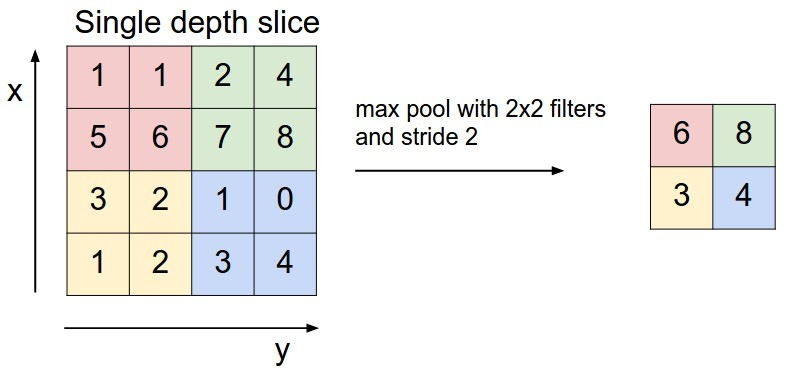
\includegraphics[width=0.5\linewidth]{figs/maxpooling.png}
          \caption{Example of max pooling operation with a 2×2 filter and a stride of 2 \cite{standfordcnn}.}
          \label{fig:maxpooling}
        \end{figure}
    \end{itemize}
    As a result of these three concepts, the overall architecture of \ac{CNN}s becomes quite different from fully connected neural networks but the same basic concepts still apply. More specifically, the main objective is still to train the weights and biases of the network such that it has good performance classifying the inputs. Additionally, previous activation functions, optimization methods, and initialization strategies can also be applied just like a normal \ac{ANN}. \par 
    
    Figure \ref{fig:cnn} illustrates a simple \ac{CNN} architecture proposed by Michael Nielsen to classify numbers from 28x28 pixel images. These images belong to the \ac{MNIST} which was first presented by LeCun \textit{et al.} \cite{LeCun1998} and is a large database of handwritten digits. This architecture has 28x28 input neurons used to encode the pixel intensities, then is followed by a convolutional layer using a $5 \times 5$ local receptive field and 3 feature maps which results in 3x24x24 feature neurons. Next, a max-pooling layer is applied with $2 \times 2$ regions of stride 2 which results in 3x12x12 hidden feature neurons. Finally, the last layer is a softmax layer and has a fully connected structure (which is not fully connected in the figure for simplicity) with 10 neurons, because the objective of the network is to classify digits between 0 and 9. \par
    \begin{figure}[ht]
      \centering
        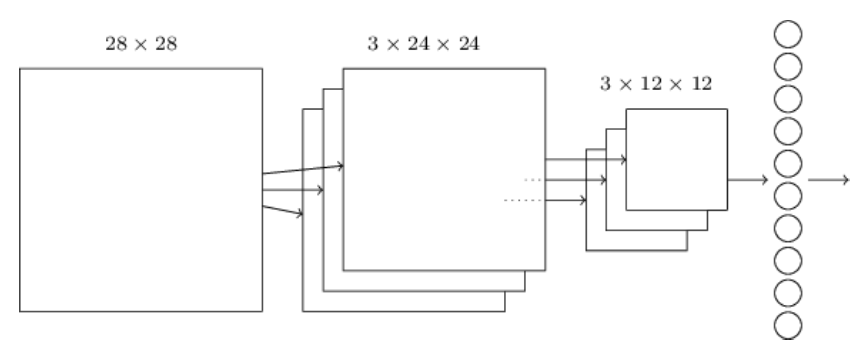
\includegraphics[width=0.7\linewidth]{figs/cnn.png}
      \caption{Custom \ac{CNN} architecture used to classify digits from the \ac{MNIST} dataset taken from Michael Nielsen \cite{Nielsen2017a}.}
      \label{fig:cnn}
    \end{figure}
    
    This represents a simple \ac{CNN} architecture for a relatively simple problem. However, more recent \ac{CNN} architectures used in large-scale data analysis problems (\textit{e.g.}, ResNet \cite{resnet}), are often more popular because of their state-of-the-art performance on different benchmarks for object recognition tasks, such as \ac{ILSVRC}. However, they are still derived from the same concepts of this simple architecture, namely, using convolution layers for feature detection, pooling layers for knowledge aggregation, and a classifier containing fully connected layers and softmax layers. \par
    
\subsection{State-of-the-art CNN Architectures}
\label{section:cnn_archs}
    Over the years several \ac{CNN} architectures have been developed and tested against benchmark challenges such as the \ac{ILSVRC} \cite{ilsvrc}. In 2012, Krizhevsky \textit{et al.} \cite{alexnet} submitted for the first time a \ac{CNN} architecture called AlexNet, which outperformed hand-crafted feature learning methods on the ImageNet dataset. It represented a significant breakthrough that leads to an increasing interest in deep learning methods for visual recognition and classification \cite{Alom2019}. It contained 8 layers, more specifically, 5 convolutional layers (some of them followed by max-pooling layers), and 3 fully-connected. This architecture also used dropout as a regularization method and the ReLU activation function, which showed improved training performance over tanh and sigmoid \cite{alexnet}. This laid the foundation for traditional \ac{CNN} architectures. \par
    
    Following AlexNet's main ideas, the VGGNet \cite{vggnet} was created and became quite popular by winning the 2014’s \ac{ILSVRC}. This architecture proved that representation depth is beneficial for the classification accuracy, as it used a traditional \ac{CNN} architecture but with increased depth along with smaller receptive fields. There are some public variations of this network, one of which has 16 weight layers (VGG16) displayed in \autoref{fig:vgg16}. This architecture is composed of multiple blocks composed of convolutional layers followed by pooling layers that progressively build more abstract features. Furthermore, this architecture employed $3 \times 3$ convolutions, $2 \times 2$ max-pooling with stride $S=2$ which meant that resolution is halved after each of these blocks. Finally, the last layer of this architecture has a fully connected structure to convert the results of the convolution into a label.  \par
    \begin{figure}[ht]
      \centering
        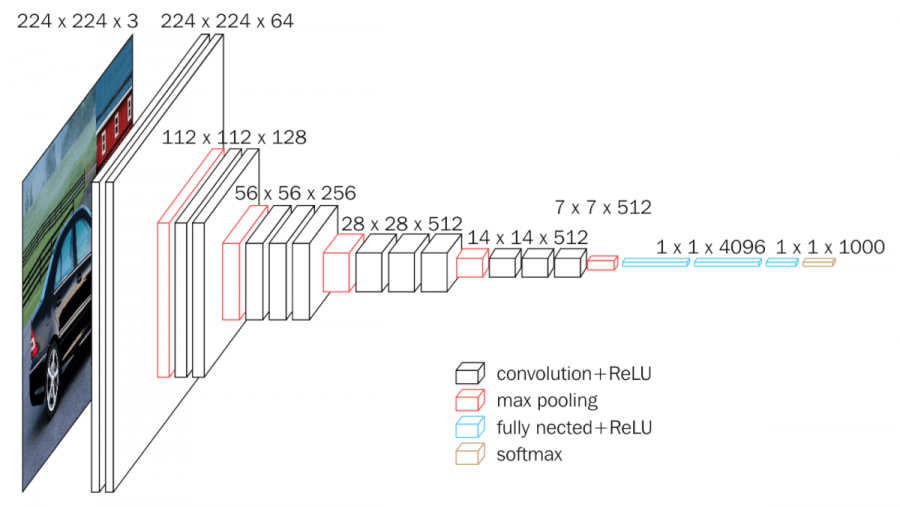
\includegraphics[width=0.8\linewidth]{figs/vgg16.png}
      \caption{Architecture of the VGG16 \ac{CNN} \cite{vggnet}.}
      \label{fig:vgg16}
    \end{figure}
    \par
    Until this point, both AlexNet and VGGNet use plain networks (\textit{i.e.}, networks that stack convolutional layers followed by fully connected layers) and both approaches explore the idea of creating deeper networks in order to obtain better performance. However, as one increases a network's depth, the problem of vanishing gradients starts to be prominent. On deep networks as the gradient is back-propagated to earlier layers, repeated multiplication may make the gradient infinitely small. Consequently, as the network becomes deeper, its performance gets saturated or even starts degrading rapidly. \par
    
    In 2015 a team of Microsoft researchers won the \ac{ILSVRC}, and later submitted a paper to the International Conference on Computer Vision and Pattern Recognition \cite{resnet}. They show that a 20 layer plain network performs better than a 56-layer plain network one due to the presence of the vanishing gradients problem on the deeper network. As such, they attempt to solve this problem with the introduction of a concept called skip connection (see \autoref{fig:skip_connection}). \par
    \begin{figure}[ht]
      \centering
        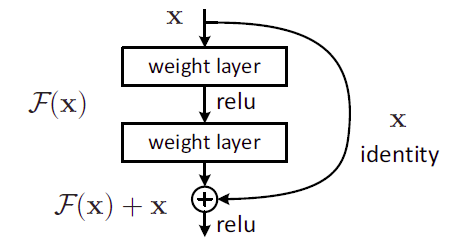
\includegraphics[width=0.5\linewidth]{figs/skip_connection.png}
      \caption{Skip connection, the building block of residual neural networks. Taken from He \textit{et al.} \cite{resnet}.}
      \label{fig:skip_connection}
    \end{figure}
    \par
    
    Consider a network with $L$ layers, where each layer of the network implements a non-linear transformation $H_l(\cdot)$, which can be seen as a composite function of operations such as convolutions, batch normalization, activation functions, or even a pooling functions. ResNets have a skip-connection that bypasses the non-linear transformations with the identity function, like the following:
    \begin{equation}
        x_l=H_l(x_{l-1})-x_{l-1}
        \label{eq:residual_mapping}
    \end{equation}
    where $x_0$ is the input image passed through the network and $x_l$ is the output of the $l$th layer.

    The advantage of this mapping is that the gradient can flow directly through the identity function from later layers to earlier layers, which ultimately helps with the vanishing gradient problem. They hypothesize that letting the stacked layers fit a residual mapping is easier than letting them directly fit the desired underlying mapping. \par
    
    More recently, Huang \textit{et al.} \cite{densenet} pointed out that whenever the output of a layer $l$ is combined with the identity function by summation, the information flow of the network may be compromised, meaning that some information might be lost in this process. Therefore, they extended the skip connection concept further in their network architecture called Dense Convolutional Network (DenseNet). Unlike ResNets, any layer has direct connections to all subsequent layers, and feature maps are combined with concatenation instead of summation. Authors argue that concatenating feature-maps learned by different layers further improve information flow efficiency and increases variation of subsequent layers. As such, in DenseNet the $l$th layer receives the feature-maps of all preceding layers. Equation \ref{eq:densenet_concatenation} mathematically shows this concept. 
    \begin{equation}
        x_l = H_l([x_0, x_1, . . . , x_{l-1}])
        \label{eq:densenet_concatenation}
    \end{equation}
    where $ [x_0, x_1, . . . , x_{l-1}] $ refers to the concatenation of the feature-maps produced in layers $ 0, . . . , l-1 $. \par
    
    Moreover, if each function $H_l$ produces $k$ feature maps, then the layer l has $k * (l- 1)$ input feature-maps, where $k_0$ is the number of channels in the inputs layer (also called growth rate). Figure \ref{fig:densenet} visually illustrates this concept, with a 5 layer dense block and a growth rate $k$ of 4.  As seen, each layer takes all preceding feature-maps as inputs. \par
    
    \begin{figure}[ht]
      \centering
        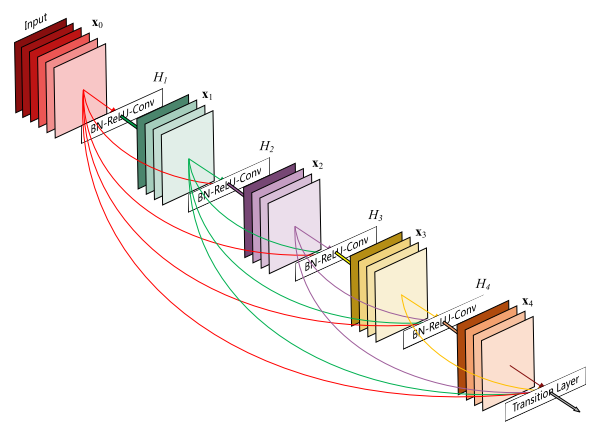
\includegraphics[width=0.8\linewidth]{figs/densenet.png}
      \caption[A block from DenseNet with five layers each with an expansion of 4]{A block from DenseNet with five layers each with an expansion of 4. Each layer combines all preceding feature maps through concatenation \cite{densenet}.}
      \label{fig:densenet}
    \end{figure}
    
    The objective of the growth rate is to regulate how much new information each layer should contribute to the global state of the network. Moreover, once the global state is written by a layer, it can be easily accessed by all the subsequent layers of the network. Therefore, contrarily to traditional neural network architectures, where there is a need to replicate the already acquired knowledge from previous layers, DenseNet is able to re-use knowledge obtained from earlier layers. \par
    
    So far, the presented architectures explore the idea of scaling up depth of the network in other to build progressively more abstract features. However, there are three dimensions in which one can scale a network (illustrated in \autoref{fig:modelscaling}): 
    \begin{itemize}
        \item Width scaling controls the width of each layer on the model (\autoref{fig:modelscaling} b). Wider networks tend to be able to capture more fine-grained features and are easier to train, but extremely wide, shallow networks tend to have difficulties in capturing higher level features \cite{efficientnet};
        \item Depth scaling controls how many layers the model has (\autoref{fig:modelscaling} c). All the former presented models explore the idea of scaling up the network in order to capture richer and more abstract features. However, issues such as the vanishing gradients problem start to be more prevalent in deeper networks. Architectures like ResNet \cite{resnet} and DenseNet \cite{densenet} attempt to solve this problem, but performance gains diminishes as models become deeper;
        \item Resolution scaling corresponds to the increase of resolution of input images (\autoref{fig:modelscaling} d). The intuition behind this type of scaling is that the network can see more detail and therefore capture more fine-grained patterns. 
    \end{itemize}
    Tan \textit{et al.} noted these three scaling dimensions are not independent. Rather, intuition tells us that for higher resolution input images, there should be a depth increase such that the larger receptive fields capture similar features that include more pixels in larger images. The authors also argue that one should increase the network width in order to capture more fine-grained patterns, because the images have more information as an input (more pixels). Following this ideas, they proposed a new family of models called EfficientNets \cite{efficientnet} which coordinates and balances different scaling dimensions together (see \autoref{fig:modelscaling} e) through the compound scaling method presented by the following expressions: \par
    \begin{equation}
        \begin{split}
            \text{depth: } d = \alpha^\theta \\
            \text{width: } w = \beta^\theta \\
            \text{resolution: } r = \gamma^\theta \\
            \text{s.t. } \alpha\cdot\beta^2\cdot\gamma^2\approx2 \\
            \text{s.t. } \alpha \geq 1, \beta \geq 1, \gamma \geq 1
            \label{eqs:efficientnetcompound}
        \end{split}
    \end{equation}
    where $\theta$ is a coefficient that controls how many resources are available for model scaling and $\alpha$, $\beta$, $\gamma$ specify how to assign these extra resources to network width, depth, and resolution respectively. All of these parameters can be optimized using grid search. \par
    
    They created a baseline model EfficientNet-B0 and then scaled up the model in three dimensions following those constraints. More specifically, 7 other models (EfficientNet-B1 to EfficientNet-B7) which increasingly have more parameters and \ac{FLOPS}, but should also have, in theory, increasingly better performance. The idea is to provide a family of models that can be adapted to one's needs, depending on the available computing capability.
    
    \begin{figure}[ht]
      \centering
        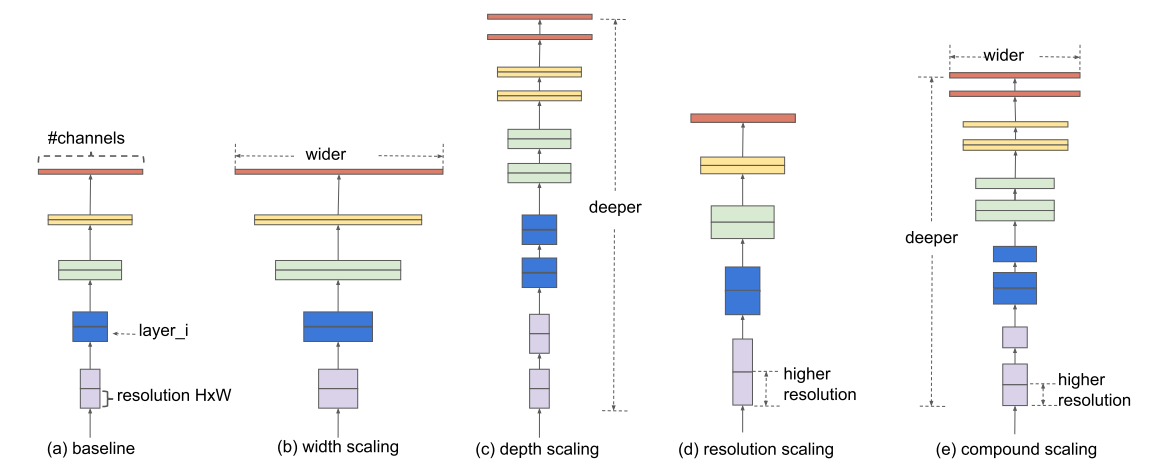
\includegraphics[scale=0.5, width=\linewidth]{figs/modelscaling.png}
      \caption{Model scaling methods as presented by Tan \textit{et al.} \cite{efficientnet}.}
      \label{fig:modelscaling}
    \end{figure}
    
    Other \ac{CNN} architectures also apply similar concepts for maximizing performance, such is the case of the Inception family of \ac{CNN} architectures. The InceptionV1 \cite{inceptionv1} (also called GoogleLeNet) was the first version of this family architecture, and explored the idea of having multiple convolutional operations but with different kernel sizes in the same layer such that different types of information are extracted in a specific layer (\textit{i.e.} information related to smaller and larger portions of the image). Therefore, the authors designed an inception module with one big filter of kernel size $5 \times 5$ for globally distributed information in the image, a medium filter of size $3 \times 3$ for slightly smaller information, a 1x1 filter for even smaller information and a $3 \times 3$ pooling layer (see \autoref{fig:inception_module}). Moreover, to make the network less computational intensive, the authors limit the number of input channels by adding an extra 1x1 convolution with a max-pooling layer before the $3 \times 3$ and $5 \times 5$ convolutions. Finally, the InceptionV1 architecture was built with 9 of such inception modules stacked on top of each other (22 layers). \par
    
    \begin{figure}[ht]
      \centering
        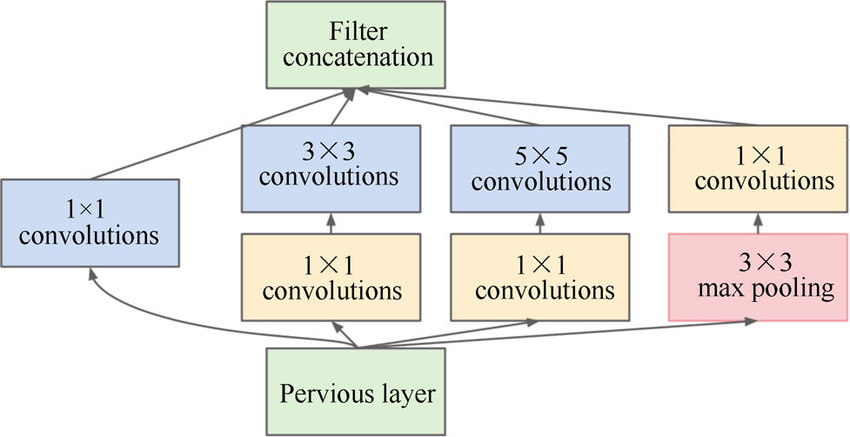
\includegraphics[width=0.6\linewidth]{figs/inception_module.png}
      \caption{Inception module from the InceptionV1 architecture \cite{inceptionv1}.}
      \label{fig:inception_module}
    \end{figure}
    
    However, like He \textit{et al.} \cite{resnet}, the authors argued that this network structure is victim of the vanishing gradients problem because it is too deep. Therefore, the authors introduced two auxiliary classifiers with softmaxes that calculated an auxiliary loss over the same labels. Finally, the total loss function is the weighted sum of the auxiliary classifiers (0.3 in the original paper) and the normal classifier. This gave rise to a far more complex architecture than ResNets or VGGNets. \par
    
    The InceptionV1 architecture was later revised by Szegedy \textit{et al.} \cite{inceptionv3}, which introduced the factorization concept in an attempt to decrease computational complexity. Factorization is a concept in which convolutions with big kernel sizes like $5 \times 5$ that are 2.78 times more expensive than $3 \times 3$ convolutions, can be reduced into the latter by having two $3 \times 3$ stacked convolutions instead. Another option is to factorize convolutions of filter size $n \times n$ to a combination of $1 \times n$ and $n \times 1$ convolutions. For example, a kernel size of $3 \times 3$ is the same as first performing a convolution of $1 \times 3$ and then perform a $3 \times 1$ convolution on the output. Taking this into account, the inception module was redone to accommodate the complexity reduction using this factorization method, which gave rise to 3 different types of inception modules called A, B and C (see \autoref{fig:inceptionv2_abc}). Furthermore, InceptionV2 overall improved the performance when compared with InceptionV1 (see \autoref{tables:pretrainedmodels}). 
    
    \begin{figure}[ht]
      \centering
        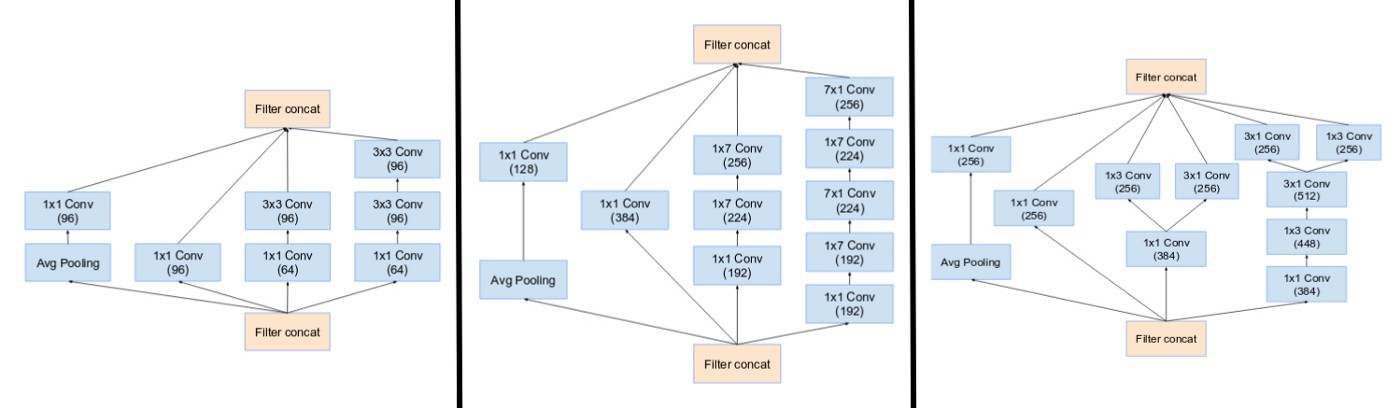
\includegraphics[width=\linewidth]{figs/inceptionv2_abc.jpeg}
      \caption{Inception module A (left), B (middle) and C (right) of the InceptionV2 architecture \cite{inceptionv3}.}
      \label{fig:inceptionv2_abc}
    \end{figure}
    
    In the same paper as the InceptionV2 approach \cite{inceptionv3}, Szegedy \textit{et al.} also proposed improvements towards the InceptionV2 architecture, which they called the InceptionV3 architecture \cite{inceptionv3}. These improvements include using the RMSProp Optimizer, $7 \times 7$ factorized convolutions, batch normalization \cite{batchnorm}, and label smoothing (\textit{i.e.}, a regularization technique added to the loss formula). \par
    
    Moreover, Szegedy \textit{et al.} revised the InceptionV3 architecture again with the premise of simplifying the modules of this architecture. This architecture is called InceptionV4 \cite{inceptionv4}, which modified the initial set of operations performed before introducing the Inception blocks. Furthermore, the authors introduced the idea of "Reduction Blocks", which are used to change the width and height of the grid. \par
    
    In the same paper, inspired by the concept of skip connection of ResNets \cite{resnet}, Szegedy \textit{et al.} proposed a hybrid inception module which integrated the skip connection concept into Inception-ResNetV1 and Inception-ResNetV2 into the inception modules A, B and C (see \autoref{fig:inceptionresnet_abc}). Inception-ResNet-V1 is similar to InceptionV3 and Inception-ResNet-V2 is similar to InceptionV4, in terms of computational complexity, as they use different hyperparameters to adjust that complexity. \par

    \begin{figure}[ht]
      \centering
        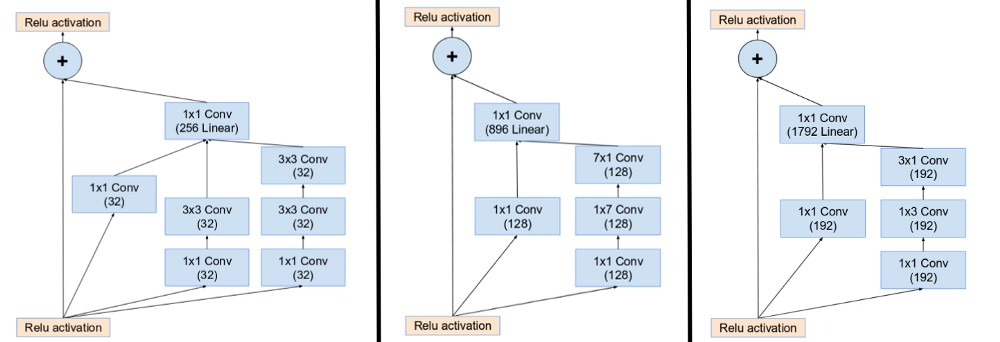
\includegraphics[width=\linewidth]{figs/inceptionresnet_abc.jpeg}
      \caption{Inception module A (left), B (middle) and C (right) of the InceptionResNet (V1 and V2) architecture \cite{inceptionv4}.}
      \label{fig:inceptionresnet_abc}
    \end{figure}
    
    % \begin{figure}[ht]
    %   \centering
    %     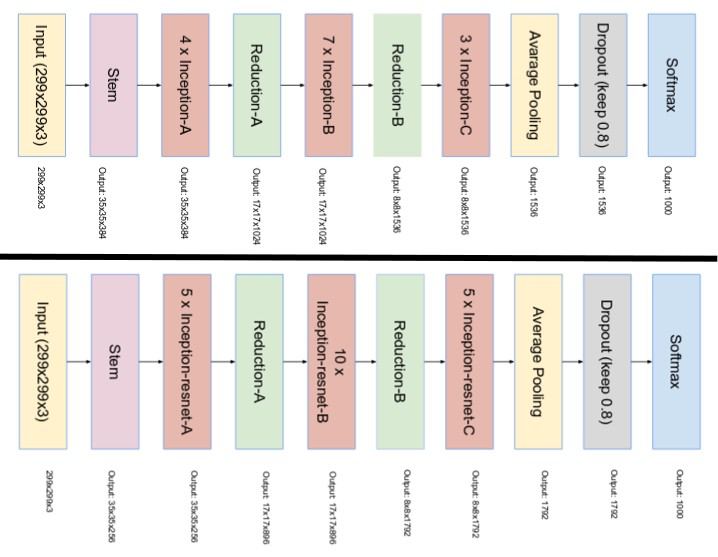
\includegraphics[width=\linewidth]{figs/inceptionv4_resnet.jpeg}
    %   \caption{InceptionV4 (top) vs. Inception-ResNet V1 and V2 (bottom) structure \cite{inceptionv4}.}
    %   \label{fig:inceptionv4_resnet}
    % \end{figure}
    
    Each of these architectures has been tested against benchmark datasets like ImageNet and their performance can be compared in \autoref{tables:pretrainedmodels}. One can observe that more recent architectures (\textit{e.g.}, EfficientNets) have significantly better accuracy scores in comparison to older ones. Furthermore, over the years, model depth and input size progressively increased, while keeping a relatively low number of trainable parameters and model size. \par 
    
    \begin{table}[h]
        \centering
        \begin{tabularx}{\textwidth}{|l|X|X|X|X|X|X|X|X|}
            \hline
            Model & Year & Size & Top-1 Accuracy & Top-5 Accuracy & Params (Millions) & Depth & Input Size \\ \hline
            AlexNet \cite{alexnet} & 2012 & 238 MB & 0.570 & 0.803 & $\approx$ 60 & 8 & 256x256 \\ \hline
            VGG16 \cite{vggnet} & 2014 & 528 MB & 0.713 & 0.901 & $\approx$ 138 & 16 & 224x224 \\ \hline
            VGG19 \cite{vggnet} & 2014 & 549 MB & 0.713 & 0.900 & $\approx$ 143 & 19 & 224x224 \\ \hline
            ResNet50 \cite{resnet} & 2015 & 98 MB & 0.749 & 0.921 & $\approx$ 26 & 50 & 224x224 \\ \hline
            ResNet101 \cite{resnet} & 2015 & 171 MB & 0.764 & 0.928 & $\approx$ 45 & 101 & 224x224 \\ \hline
            ResNet152 \cite{resnet} & 2015 & 232 MB & 0.766 & 0.931 & $\approx$ 60 & 152 & 224x224 \\ \hline
            ResNet50V2 \cite{resnetv2} & 2016 & 98 MB & 0.760 & 0.930 & $\approx$ 26 & 50 & 224x224 \\ \hline
            ResNet101V2 \cite{resnetv2} & 2016 & 171 MB & 0.772 & 0.938 & $\approx$ 45 & 101 & 224x224 \\ \hline
            ResNet152V2 \cite{resnetv2} & 2016 & 232 MB & 0.780 & 0.942 & $\approx$ 60 & 152 & 224x224 \\ \hline
            DenseNet121 \cite{densenet} & 2016 & 33 MB & 0.750 & 0.923 & $\approx$ 8 & 121 & 224x224 \\ \hline
            DenseNet169 \cite{densenet} & 2016 & 57 MB & 0.762 & 0.932 & $\approx$ 14 & 169 & 224x224 \\ \hline
            DenseNet201 \cite{densenet} & 2016 & 80 MB & 0.773 & 0.936 & $\approx$ 20 & 201 & 224x224 \\ \hline
            InceptionV3 \cite{inceptionv3} & 2015 & 92 MB & 0.779 & 0.937 & $\approx$ 24 & 159 & 299x299 \\ \hline
            InceptionResNetV2 \cite{inceptionv4} & 2016 & 215 MB & 0.803 & 0.953 & $\approx$ 56 & 572 & 299x299 \\ \hline
            EfficientNetB0 \cite{efficientnet} & 2019 & 5.3 MB & 0.773 & 0.935 & $\approx$ 5 & NA & 224x224 \\ \hline
            EfficientNetB1 \cite{efficientnet} & 2019 & 7.9 MB & 0.792 & 0.945 & $\approx$ 8 & NA & 240x240 \\ \hline
            EfficientNetB2 \cite{efficientnet} & 2019 & 9.2 MB & 0.803 & 0.950 & $\approx$ 9 & NA & 260x260 \\ \hline
            EfficientNetB3 \cite{efficientnet} & 2019 & 12.3 MB & 0.817 & 0.956 & $\approx$ 12 & NA & 300x300 \\ \hline
            EfficientNetB4 \cite{efficientnet} & 2019 & 19.5 MB & 0.830 & 0.963 & $\approx$ 19 & NA & 380x380 \\ \hline
            EfficientNetB5 \cite{efficientnet} & 2019 & 30.6 MB & 0.837 & 0.967 & $\approx$ 30 & NA & 456x456 \\ \hline
            EfficientNetB6 \cite{efficientnet} & 2019 & 43.3 MB & 0.842 & 0.968 & $\approx$ 43 & NA &456x456 \\ \hline
            EfficientNetB7 \cite{efficientnet} & 2019 & 66.7 MB & 0.844 & 0.971 & $\approx$ 66 & NA &600x600 \\ \hline
        \end{tabularx}
        \caption[Models comparison on the ImageNet dataset.]{Models comparison on the ImageNet dataset. This comparison is made based on top-1 and top-5 accuracy scores towards the ImageNet validation dataset and entries are chronologically ordered.}
        \label{tables:pretrainedmodels}
    \end{table} 


\section{Transfer Learning}
\label{section:mam_transfer_learning}
    Training deep neural networks from scratch is often a difficult process because it requires:
    \begin{itemize}
        \item Large amounts of labeled data that closely resembles the field it tries to describe; 
        \item Time to train which is largely dependent on the computational power available;
        \item Ability to reason about hyperparameters and follow heuristics to achieve a good model on the cross-validation process.
    \end{itemize}
    
    However, these requirements can be quite difficult to attain especially for small teams with limited monetary and human resources. Particularly, in the medical imaging context, public datasets to train deep networks are rather scarce \cite{Miotto2017}. Even when one has a good dataset along with high computational power, the training process can take a long time, especially while debugging the network to determine a good model fit. \par
    
    Transfer learning emerged as a way of relaxing the need for the aforementioned requirements. Transfer learning is a method of reusing a pre-trained model's knowledge for another related task \cite{DipanjanSarkarRaghavBali2018}. Using transfer learning means to carry the parameters from a model trained on a generic dataset (\textit{e.g.}, ImageNet), and leveraging it to re-train the model for a different purpose. Moreover, a pre-trained model is a model that was already trained in some domain and can be somehow adapted to a similar domain. For example, if one needs to recognize cats or dogs in an image, instead of training the VGG16 architecture from scratch, one can use the VGG16 pre-trained model (on ImageNet) and leverage the previous weights for the new recognition task. \par
    
    In \ac{CNN}s, as inputs are passed along the network, hidden layers closer to the input layer output generic features like shapes and curves, while hidden layers closer to the output layers build more abstract features such as a dog's face. In order to adapt the pre-trained models into a different domain, one must extract the parameters up to some layer from the pre-trained model while freezing (\textit{i.e.}, to not allow parameter updates while training) some or no portion of those layers. \par
    
    In order to repurpose the knowledge from a pre-trained model, the classifier must be replaced by a classifier that fits one's needs, while keeping the rest of the architecture (called the convolutional base) intact. Figure \ref{fig:transferlearning} illustrates three different strategies to repurpose a pre-trained model:
    \begin{itemize}
        \item Strategy 1: Fine-tune the whole model. This means to extract all weights from the convolutional base and fine-tune them along with the classifier's weights. It often requires both more computational power, because it has more parameters to train, and more data to adapt the model to its new purpose;
        \item Strategy 2: Freeze part of the model while fine-tuning the remaining layers. As previously mentioned lower layers identify problem independent features, while higher layers refer to problem-dependent features. As such, one can choose up to which layer should the model be frozen, depending on how much different the problem is compared to the original pre-trained model's problem. Some general advice can be given about this type of strategy. If the dataset to train the pre-trained model is big and similar to the original dataset then fine-tuning fewer layers (only the last layers) will likely yield better performance. However, if one has a small target dataset which is fairly different from the original dataset in which the pre-trained model was trained on, then fine-tuning most of the layers (except the first ones) might grant better results;
        \item Strategy 3: Keep the same convolutional base parameters and only train the classifier. Usually used in cases where the purpose of the pre-trained model is very similar to the problem that one is trying to solve, meaning that the two datasets are similar. This can be a good strategy if the available computational power is low because the only parameters required to train are the ones from the classifier layers.
    \end{itemize}
    
    \begin{figure}[ht]
      \centering
        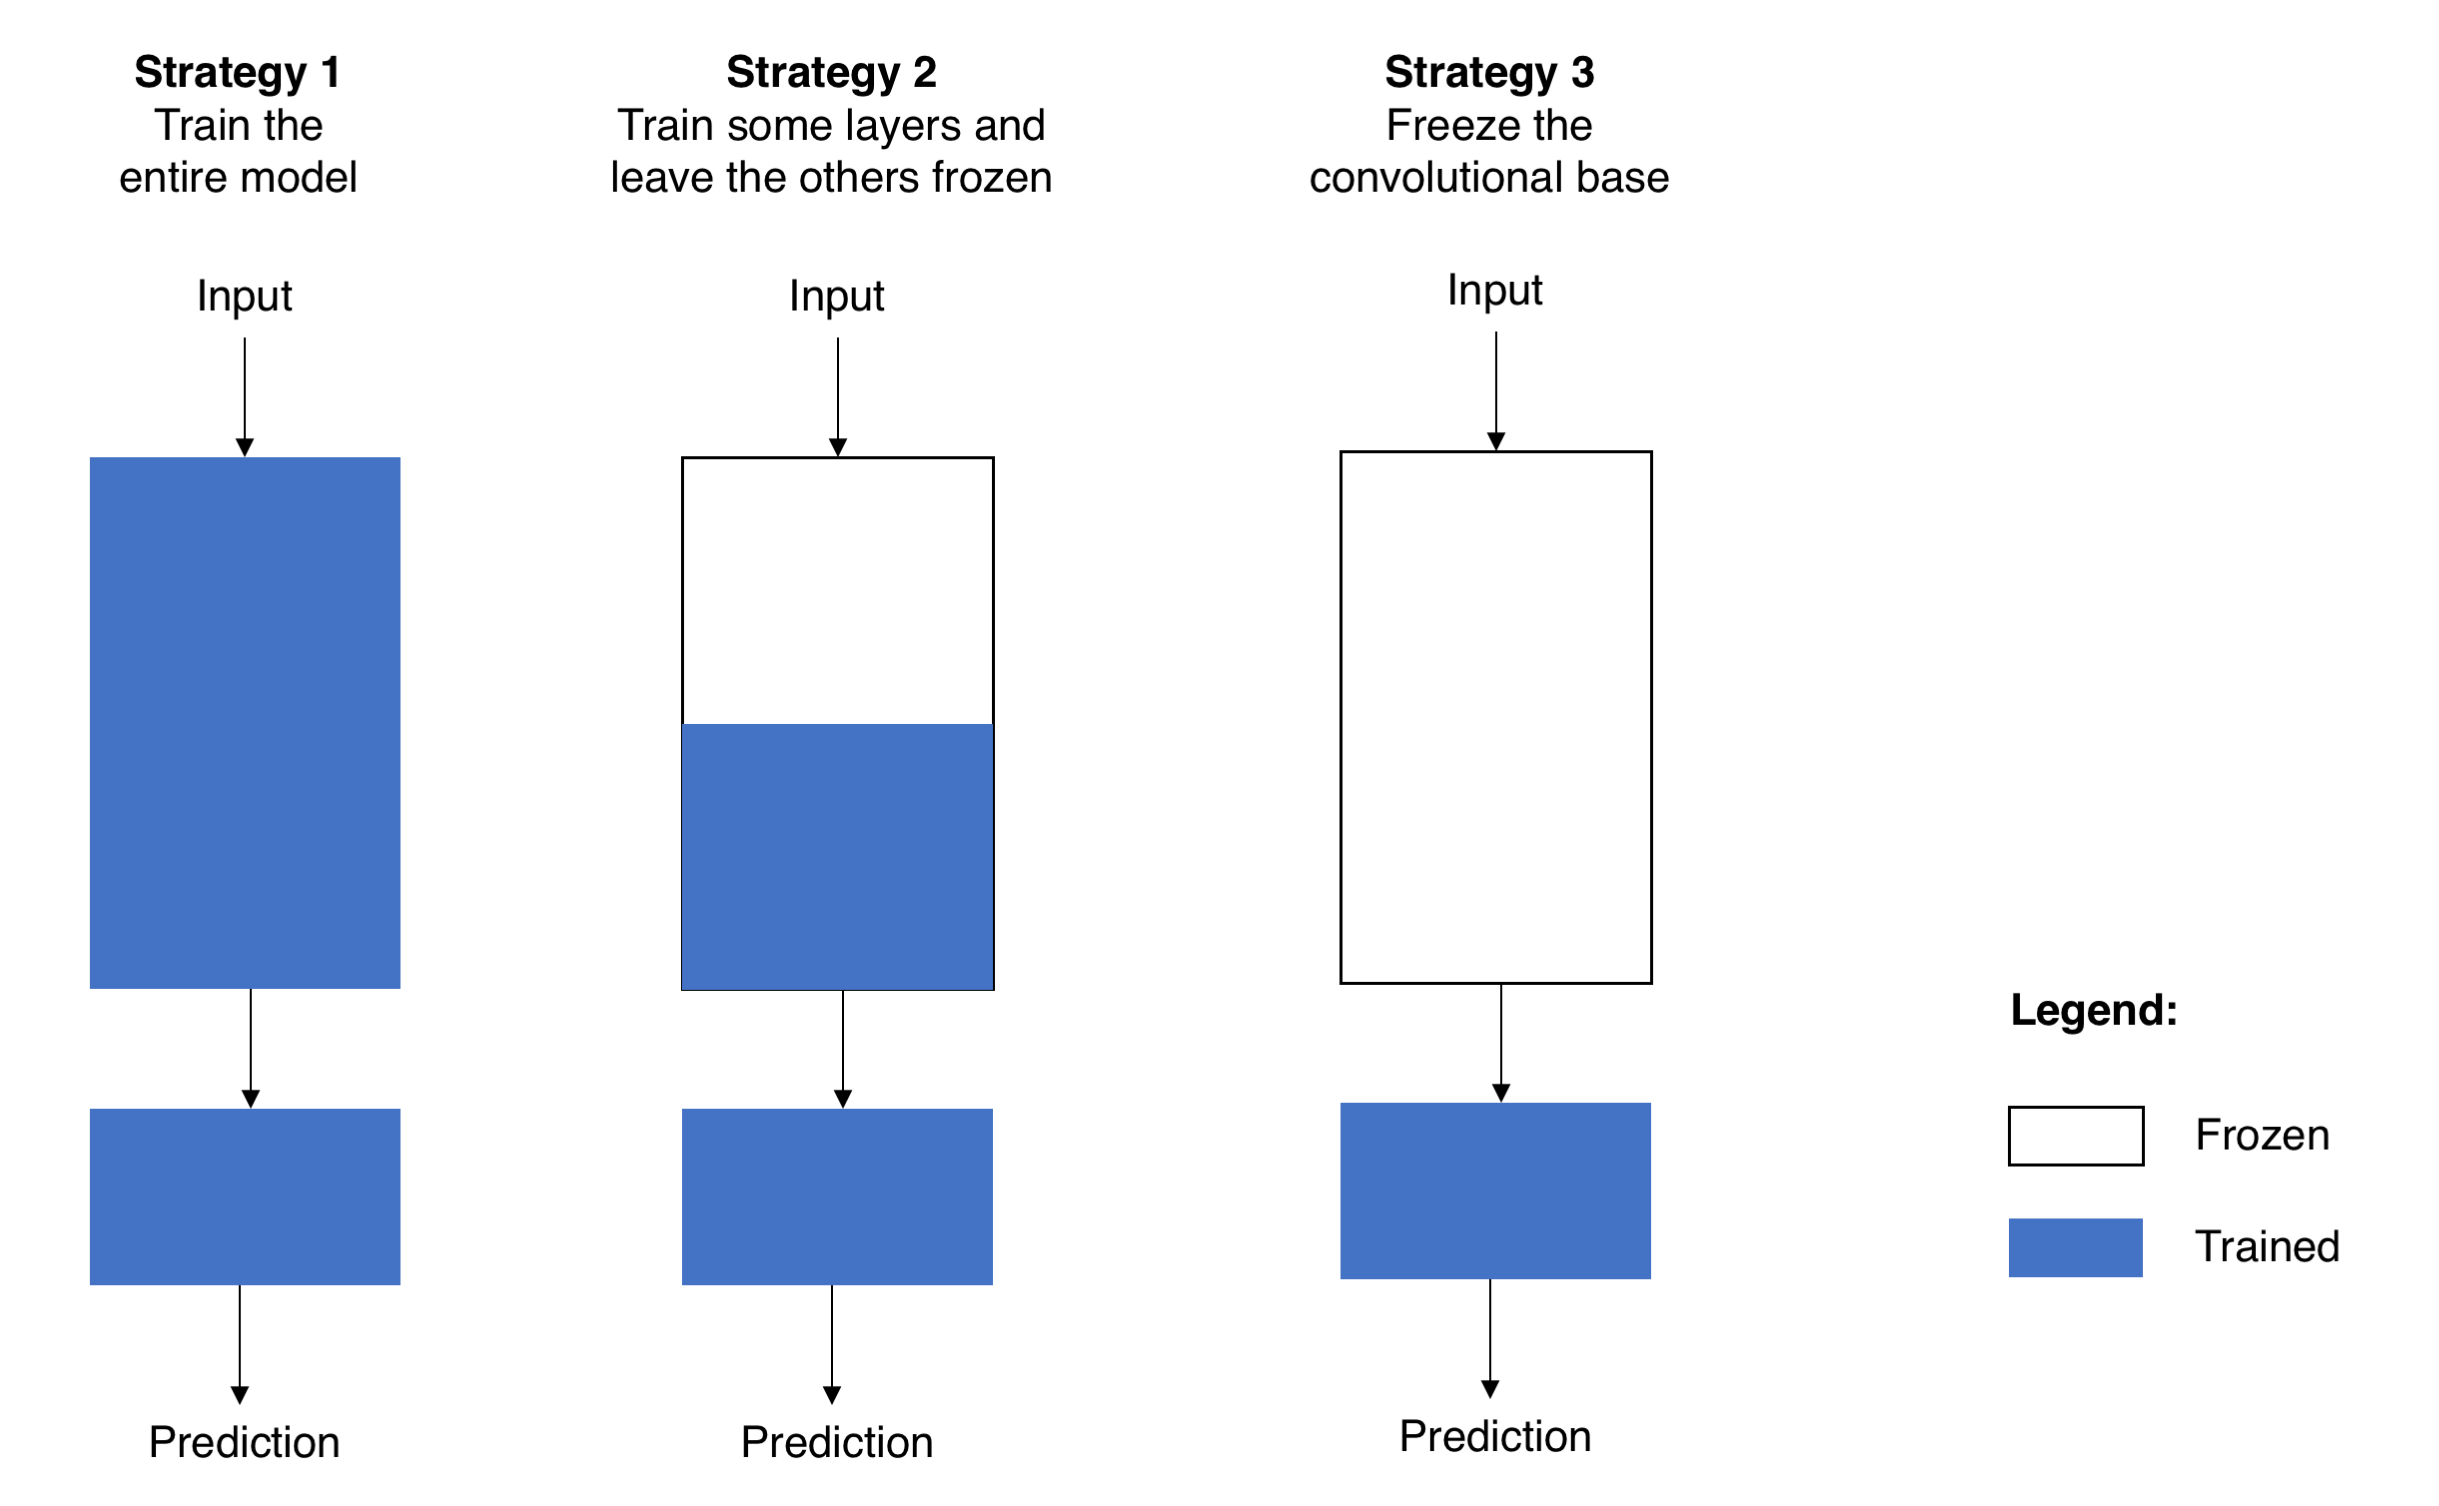
\includegraphics[scale=0.5, width=\linewidth]{figs/transfer_learning.png}
      \caption[Transfer learning strategies]{Transfer learning strategies as described by Pedro Marcelino \cite{marctransferlearning}.}
      \label{fig:transferlearning}
    \end{figure}
    
    In \ac{CNN}s, while the convolutional base works as a feature extractor, the classifier uses the features extracted by the convolutional base in order to classify the input. Different options can be used to replace the original classifiers used on the pre-trained models, namely: 
    
    \begin{itemize}
        \item Fully-connected layers followed by a softmax layer, which is the standard approach \cite{alexnet}. The softmax layer outputs the probability distribution over each class label and the classification is equal to the most probable class;
        \item First proposed by Lin \textit{et al.} \cite{lin2013network}, one can add a global average pooling layer at the end of the convolutional base, followed by a softmax layer; 
        \item Finally, according to Tang \cite{Tang2013}, one can improve classification accuracy by training a linear \ac{SVM} classifier on the features extracted by the convolutional base. 
    \end{itemize}

\section{The Bias and Variance Tradeoff}
\label{section:overfitting_underfitting}
    While training, one must fine-tune the model to both accurately make predictions from the training data while generalizing to new data. The bias and variance tradeoff is a well-known problem in deep learning that represents a tradeoff between these two requirements. While the bias of a model is the error caused by the assumptions made to approximate the model to the true predictions, the variance of a model is the error from sensitivity to small fluctuations in the training set. One must find a good tradeoff between bias and variance so that the model does not underfit or overfit (see \autoref{fig:biasvariancetradeoff}). \par
    
    \begin{figure}[ht]
      \centering
        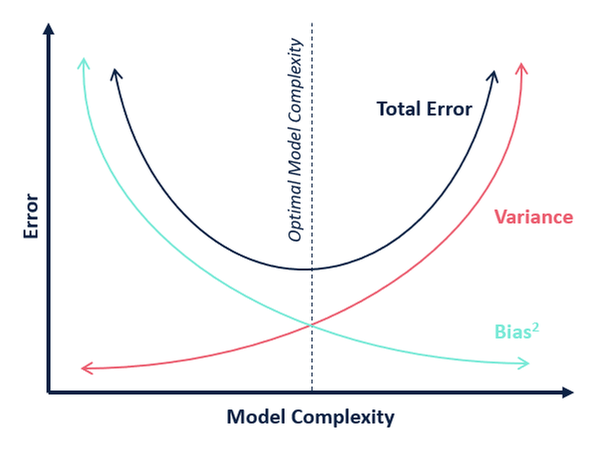
\includegraphics[width=0.5\linewidth]{figs/bias_variance_tradeoff.png}
      \caption[Influence of model complexity on the bias and variance.]{Influence of model complexity on the bias and variance. As the complexity of the model rises, the bias of the model decreases but the variance increases. One should find the optimal point of model complexity for a good bias and variance tradeoff, in order to minimize the model's total error.}
      \label{fig:biasvariancetradeoff}
    \end{figure}
    
    If the model underfits, then it does not perform well even on the training data, and therefore has high bias and low variance. However, the opposite can also happen, more specifically, producing a model that performs well on the training data but that generalizes poorly to new data \cite{Grus}. In this case, the model overfits and therefore has a low bias, but very high variance. In order to evaluate whether a model is underfitting or overfitting, one should use metrics that help describe what is happening while training (see \Cref{section:metrics}). \par  
    
    \subsection{Underfitting Solutions}
    \label{section:underfitting}
    
    A larger neural network can, generally, reduce underfitting because it has more parameters that can be adapted to a specific function and, therefore, minimize the bias of the model (see \autoref{fig:biasvariancetradeoff}). In order to add new parameters to the model, one can increase the depth of the network (more layers) or increase the neurons per layer (wider layers). \par
    
    An alternative option to deal with underfitting is to increase the number of epochs such that the model eventually finds the optimal trainable parameters to minimize the loss (\textit{e.g.}, increase the early stopping requirements). Finally, one can also reduce the impact of the regularization being applied which would ultimately lead to a better adaptation of the model to the training dataset. \par
    
    \subsection{Overfitting Solutions}
    \label{section:overfitting}
    Multiple solutions to the overfitting problem have been proposed and tested over the years. Presumably the most intuitive is to reduce the network’s capacity by removing layers or reducing the number of elements in the hidden layers. This will help because the network will have fewer parameters to learn and therefore minimize the chance of the network memorizing inputs, which leads to a high variance scenario (see \autoref{fig:biasvariancetradeoff}). \par
    
    Other ways of dealing with this problem are the regularization techniques, which are broadly described by some authors as any method that allows the model to further improve generalization performance \cite{Nielsen2017a}. For example, while L1 and L2 regularization attempt to create less complex models \cite{Ng}, techniques such as dropout "reduce complex co-adaptations between neurons" \cite{Hinton2012}, by randomly removing nodes from a specific layer of the network. Alternatively, techniques such as batch normalization can be used to normalize the set of activations in a layer. It works by subtracting the mean from each batch to each activation and then dividing it by the standard deviation from that batch \cite{batchnorm}. \par
    
    When a model keeps improving training performance but does not improve validation performance at the end of the training process, it generally means that the model is memorizing the training set rather than learning generalizable features. In this context, early stopping can help reduce overfitting as it stops the model from training further whenever validation performance stagnates for several epochs. \par
    
    In deep learning, a model is highly dependent on its training dataset in order to achieve good generalization performance \cite{Shorten2019}. For example, if a dataset does not provide enough proper real-world variation or size or both, then it can easily cause the network to memorize inputs (overfitting). In contrast, a relatively big dataset, representative of the real-world samples, and with enough diversification will force the model to optimize weights towards generalized knowledge rather than memorize inputs. \par
    
    However, when one does not have a proper dataset available, a concept called data augmentation can be used to alleviate this requirement. The main idea behind this concept is to expand the training data by applying operations that reflect real-world variation to original samples \cite{Nielsen2017a}. Shorten \textit{et al.} \cite{Shorten2019} provides a comprehensive survey about different image processing techniques that can be used for data augmentation, from simple transformations such as translations, rotations, or flips to more complex transformations like distortions or region erasing. Another alternative is to synthetically create new samples through methods like \ac{GAN}s, which is a type of neural network. \par 
    
    Moreover, there are two main ways of applying data augmentation for training deep neural networks:
    \begin{itemize}
        \item Offline data augmentation, in which images are generated before the training process and stored in disk for the training of the neural network. This approach can be useful if one wants to employ some kind of schema to apply data augmentation to a particular set of images (\textit{e.g.}, class balance samples). However, it can become troublesome if one has limited disk space, as it increases the storage requirements;
        \item Online data augmentation, in which images are generated per iteration during training, and differ in each epoch. In other words, in each epoch, the network is going to be fed a different variation of the original image, rather than the same image. This means that images are created in each epoch iteration and stored in memory for the duration of the iteration and deleted at the end. The big advantage of this approach is related to the lack of requirements for additional disk space to store additional images. However, if the augmentation techniques are rather slow, the training process can take longer. Additionally, it is rather difficult to filter which samples should be augmented according to a schema in this approach. 
    \end{itemize}

\section{Ensemble Learning}
\label{section:ensemble_learning}
    Neural networks are non-linear methods, which means that they can learn complex non-linear relationships in the data. A downside of this flexibility is that they are sensitive to initial conditions, both in terms of the initial random weights and in terms of the statistical noise in the training dataset \cite{Brownlee}. As such, depending on the initial conditions, neural networks may learn a very different version of the mapping function from inputs to outputs, which will directly impact the model's performance. \par
    
    One option to deal with this issue is by using ensemble learning, which is a machine learning paradigm that combines multiple weak learners (models) that solve a particular problem in order to create a presumably better performing model. These are called weak learners because they often suffer from either high bias which usually happens to low complexity algorithms (\textit{e.g.}, linear regression) or high variance which is associated with high complexity algorithms (\textit{e.g.}, neural networks). Ensemble learning is a studied field that provides several methods to combine different models, and this work will present a few common ones. \par

\subsection{Combine Models Trained on Different Data}
    If the data used to train each member of the ensemble is different, then different models will be produced and the ensemble will presumably yield better performance. This work highlights two options to combine models with different data: 
    \begin{itemize}
        \item Ensemble the models created with k-fold cross-validation: In this procedure, given a dataset with $n$ samples, $k$ different models are trained on $k$ different subsets of the data, with each set of training data having $n-\frac{n}{k}$ samples where the $k$th set of data is the test set with $\frac{n}{k}$ samples. These models can then be saved and used as members of an ensemble;
        \item Bagging (short for bootstrap aggregating): Given a training dataset with size $n$, bagging generates $m$ new training sets each of size $k$, by sampling from the original dataset uniformly with replacement (observations may be repeated). Then, $m$ models are fitted using the $m$ bootstrap samples and are combined by averaging the output for regression problems or voting for classification problems.
    \end{itemize}
    
\subsection{Combine Models Trained on Different Conditions}
    Training neural networks with different initial conditions will result in different models. This means that one can vary those initial conditions and combine the resulting models (ensemble) in order to reduce the variance (overfitting). \par
    
    A possible approach for this would be to use a different set of hyperparameters (\textit{e.g.}, learning rate or loss function used) or even a different set of model architectures. This will hopefully create an ensemble of models that are going to learn substantially different mapping functions between inputs and outputs, which will lower the correlation between predictions. \par
    
    An alternative to this method is to periodically save the best model during training and then ensemble those models. This method is called snapshot ensembling, described by Huang \textit{et al.} as an optimization process that visits several local minimums before converging to a final solution \cite{snapshot}. A variation for this method is to save models from a range of epochs, perhaps identified by reviewing learning curves \cite{horizontalvertical}. \par
        
    Stochastic gradient descent with warm restarts \cite{sgdr} is another variation in which the optimization procedure is changed during training (\textit{e.g.}, oscillating the learning rate). Afterwards, the best models are saved on specific checkpoints and their predictions are combined. \par
    
\subsection{Combine Predictions from Different Models}
    The following are some of the methods to combine different model's predictions:
    \begin{itemize}
        \item Average the results from all models, which in neural networks often means to average the softmax probabilities;
        \item Create a new model that learns how to combine the predictions of the different ensemble models, which is often called model stacking;
        \item Boosting, in which ensemble members are added one at a time in order to correct the mistakes of prior models;
        \item Model weight averaging \cite{Izmailov2018}, which attempts to average the weights of neural networks with the same architecture, rather than their predictions in an attempt to obtain a slightly more optimized model.
    \end{itemize}

\section{Performance Metrics}
\label{section:metrics}
    In order to assess whether or not a deep learning model has good train and generalization performance, one should use metrics to quantify the results. In this context, for binary classification one can use the following basic measures:
    \begin{itemize}
        \item \ac{TP}, cases correctly classified as positive;
        \item \ac{TN}, cases correctly classified as negative;
        \item \ac{FP}, cases incorrectly classified as positive;
        \item \ac{FN}, cases incorrectly classified as negative.
    \end{itemize}
    
    One can derive the following metrics from the presented measures:
    \begin{itemize}
        \item \ac{TPR} (also known as sensitivity or recall) is the percentage of true positives that are classified as positive:
        \begin{equation}
            TPR = \frac{TP}{TP + FN}
            \label{eq:tpr}
        \end{equation}
        
        \item \ac{TNR} (also known as specificity), is the percentage of true negatives that are classified as negative:
        \begin{equation}
            TNR = \frac{TN}{FP + TN}
            \label{eq:tnr}
        \end{equation}
        
        \item \ac{PPV}, which is also known as precision:
        \begin{equation}
            PPV = \frac{TP}{TP + FP}
            \label{eq:ppv}
        \end{equation}
        
        \item \ac{NPV}:
        \begin{equation}
            NPV = \frac{TN}{TN + FN}
            \label{eq:npv}
        \end{equation}
        
        \item \ac{FPR}, which is the percentage of true positives that are classified as negative:
        \begin{equation}
            FPR = 1 - TNR
            \label{eq:fpr}
        \end{equation}
    \end{itemize}
    
    For a multi-class classification problem, the above notions can be applied to each label independently to get a per-class metric or be averaged out across all classes, such that a single metric becomes representative of the per-class metrics. \par
    
    A commonly used metric in the context of deep learning is the accuracy $A$, also known as the fraction of correct predictions. Consider that there are $n$ samples in a dataset, where $\hat{y}_i$ is the predicted value and $y_i$ is the true value of the $i$th sample, then the accuracy can be described by: 

    \begin{equation}
        A = \frac{1}{n} * \sum_{i=0}^{n} 1(\hat{y}_i = y_i) 
        \label{eq:acc}
    \end{equation}
    where $1(x)$ is the indicator function (\textit{i.e.}, a random variable that takes value 1 when the event happens and value 0 when the event does not happen). \par
    
    However, one should not use the accuracy as the main metric when there is a high class imbalance, because the model can make a lot of correct predictions towards classes with the majority of the samples, classify incorrectly samples from minority classes and still have considerably high accuracy. As such, other metrics that take into account each class's performance as equal such as the Balanced Multi-class accuracy (\ac{BMA}), should be used:
    
    \begin{equation} 
        BMA = \frac{1}{C} * \sum_{i=0}^{C} TPR_i 
        \label{eqs:bma}    
    \end{equation}
    where $C$ is the number of classes. This metric is the macro-average of the per-class recall, but can also be seen as the accuracy where each sample is weighted according to the inverse pervasiveness of its true class. The \ac{BMA} score is the same as the accuracy for balanced datasets or when the classifier performs equally well across all classes. 
    
    Another frequently used metric is the \ac{AUC} or the area under the \ac{ROC} curve. A \ac{ROC} curve is a plot that illustrates the performance of a binary classifier system as its discrimination threshold is varied. It is created by plotting the \ac{TPR} vs. \ac{FPR}, at various threshold settings (see example in \autoref{fig:auc_roc}). The \ac{AUC} (also known as AUROC) function summarizes the curve information in one number by computing the area under the receiver operating characteristic (ROC) curve. For multi-class classification problems, the \ac{ROC} curve can be micro or macro averaged (see example in \autoref{fig:auc_roc}) to compute a single \ac{AUC} score representative of the classifier's performance across all classes. \par
    
    \begin{figure}[ht]
      \centering
        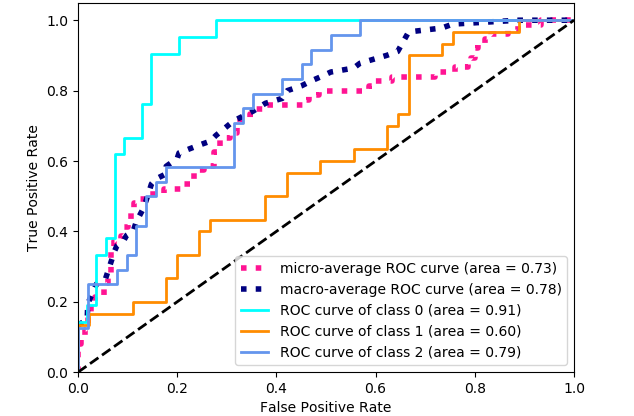
\includegraphics[width=0.6\linewidth]{figs/aucroc.png}
      \caption[ROC (Receiver Operating Characteristic) curve for a multi-class classification problem with micro and macro averages to summarize all classes. Taken from scikit-learn.]{ROC (Receiver Operating Characteristic) curve for a multi-class classification problem with micro and macro averages to summarize all classes. Taken from scikit-learn\footnotemark .}
      \label{fig:auc_roc}
    \end{figure}
    
    For all of the above metrics or even more complex ones, the values can be derived from the confusion matrix. A confusion matrix is a tabular way of visualizing the performance, where each entry $i,j$ is the number of observations from group $i$ (true label), but are predicted to be in group $j$ (\textit{e.g.}, left side of \autoref{fig:conf_matrix_example}). A confusion matrix can also be normalized, which allows to report ratios instead of counts. To normalize a confusion matrix, one must divide each entry by the sum of the counts per row (\textit{e.g.}, right side of \autoref{fig:conf_matrix_example}).
    
    \begin{figure}[ht]
      \centering
        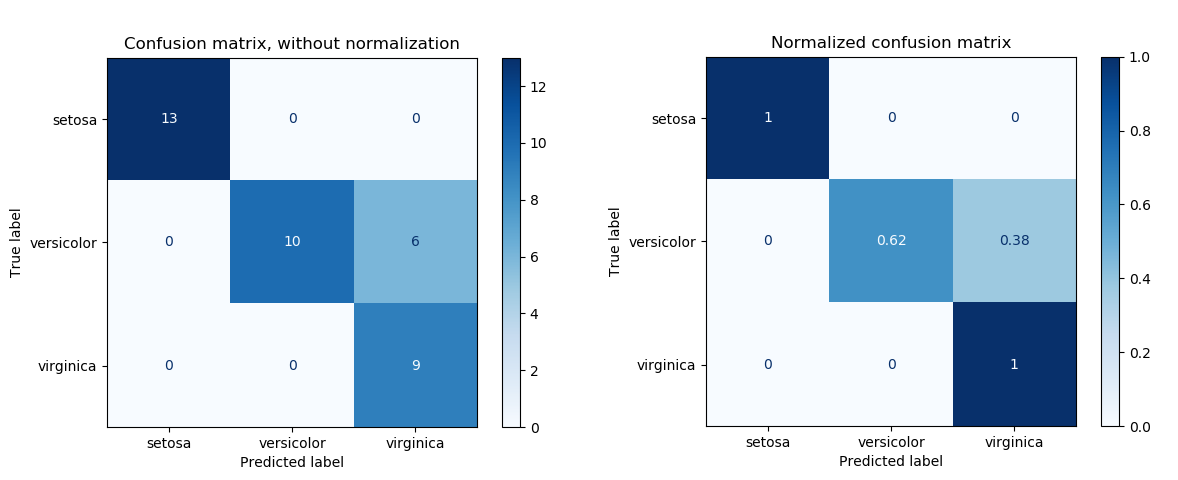
\includegraphics[width=\linewidth]{figs/conf_matrix_example.png}
      \caption{Non-normalized vs. normalized confusion matrix for a 3 class classification problem. Taken from scikit-learn.}
      \label{fig:conf_matrix_example}
    \end{figure}
    
    \footnotetext{\url{https://scikit-learn.org/stable/modules/model_evaluation.html}}
    
\section{Out of Training Distribution Detection}
\label{section:out_of_distribution}
    When machine learning classifiers are employed in real-world tasks, they will often fail if the training and test distributions differ, and, sometimes they provide high confidence predictions while being severely incorrect \cite{Goodfellow2015}\cite{Amodei2016}. This is a known problem of deep neural networks which severely limits their adoption in real-world scenarios \cite{Hendrycks2019}. Furthermore, this problem has already appeared in the literature in practical classification tasks. For example, Tschandl \textit{et al.} reports that a deep learning model trained to classify skin lesions significantly drops performance when the test data is from a different dataset from the train data \cite{humanvsisic2018}. 
    
    Mathematically, one can frame this problem as: Let $P_X$ and $Q_X$ denote two substantially different data distributions defined on the image space $Y$. Furthermore, assume that a neural network $f$ is trained with the dataset drawn from the distribution $P_X$. In this example, one can call $P_X$ the in-distribution and $Q_X$ the out-distribution. In testing, new images are drawn from a mixture distribution $P_{X \times Z}$ defined on $Y \times \{0, 1\}$, where the conditional probability distributions $P_{X|Z=0}=P_X$ and $P_{X|Z=1}=Q_X$ denote in- and out-distribution respectively. Given an image $X$ drawn from the mixture distribution $P_{X \times Z}$, out of distribution detection methods aim to assess whether the image is from in-distribution $P_X$ or not. \par
    
    A naive approach for detecting out-of-distribution samples is to train the model with a new class composed of samples belonging to a different distribution. However, the extent of the out-of-distribution examples can be too large and it requires the network to be retrained with such samples. Furthermore, it can be difficult to aggregate a set of samples not present in the training distribution which represent that class in a real-world scenario.  Moreover, this approach would require a more complex model (\textit{i.e.}, with more trainable parameters) in order to deal with the set of heterogeneous samples present in the out of distribution class. Otherwise, problems related to underfitting could occur which highlights some of the limitations to the practicality of this approach. \par

    In contrast, Hendrycks and Gimpel \cite{Hendrycks2019} noted that pre-trained neural networks can be overconfident to out-of-distribution samples even if those samples are irrelevant or unrecognizable. As such, they proposed a baseline method to detect out-of-distribution examples without further re-training networks. The method is based on an observation that a well-trained neural network tends to assign higher softmax scores to in-distribution examples than out-of-distribution examples. In practice, this means that samples should be classified as out-of-distribution if their highest softmax score is lower than a certain threshold. Furthermore, this approach served as a baseline method for future implementations of out-of-distribution detectors.  \par
    
    More recently, Liang \textit{et al.} (a team of Facebook researchers), tried to improve this baseline method with a new detector which they called \ac{ODIN} \cite{odin}. It is based on two main concepts that further increases the gap between the softmax scores of in and out of distribution samples, namely:
    \begin{itemize}
        \item Consider a neural network $f$ trained to classify $N$ classes, such that $f = (f_1, ..., f_N)$. For each input x, the neural network assigns a label $\hat{y}(x) = argmax_{i} S_{i}(x; T)$ by computing the softmax output for each class. Equation \ref{eqs:temperature_scaling} shows the adjusted softmax.
        \begin{equation}
            S_i(x; T) = \frac{exp(f_i(x)/T)}{\sum_{j}^{n}exp(f_j(x)/T)}
            \label{eqs:temperature_scaling}
        \end{equation}
        where $T \in \mathbb{R}^{+}$ is the temperature scaling parameter and set to 1 during the training. For a given input $x$, the softmax score (or the maximum softmax probability) is given by $S_{\hat{y}}(x; T) = max_i S_i(x; T)$.
        
        By tuning $T$, one can increase the gap between softmax scores of in and out of distribution samples in the test set. Moreover, according to Hinton \textit{et al.} adding temperature scaling to the softmax function will distill the knowledge of the neural network \cite{Hinton2015} as well as provide a way to calibrate the prediction confidence in classification tasks \cite{Guo2017};
        
        \item Goodfellow \textit{et al.} noted that small perturbations added to samples before prediction tend to decrease the softmax score for the true label and force the neural network to make a wrong prediction \cite{Goodfellow2015}. This also reflects into out of distribution detection, as these perturbations can have a stronger effect on the in-distribution images than that on out-of-distribution images. This concept is leveraged by ODIN as a way to further make in and out of distribution samples more separable through the \autoref{eqs:odin_perturbations}.
        \begin{equation}
            \widetilde{x} = x-\varepsilon sign(-\nabla_{x} log S_{\hat{y}}(x;T))
            \label{eqs:odin_perturbations}
        \end{equation}
        where the parameter $\varepsilon$ can be interpreted as the perturbation magnitude.
    \end{itemize}
    The \ac{ODIN} detector works by obtaining the preprocessed image $\widetilde{x}$ according to the \autoref{eqs:odin_perturbations}, then feed the result into the neural network and calculate its softmax score $S(\widetilde{x}; T)$. Finally, one should compare the obtained score with a pre-defined threshold $\delta$ so that images that are part of the in distribution dataset, have a softmax score above the threshold. Otherwise, they are predicted to be an out of training distribution sample. (see \autoref{eqs:odin_threshold}). 
    \begin{equation}
        g(x; \delta, T, \varepsilon) = \begin{cases} 1, & \mbox{if } max_{i}p(\widetilde{x};T) \leq \delta \\ 0, & \mbox{if } max_{i}p(\widetilde{x};T) > \delta \end{cases}
        \label{eqs:odin_threshold}
    \end{equation}
    where $T$, $\varepsilon$ and $\delta$ are chosen so that the \ac{TPR} (\textit{i.e.}, the fraction of in-distribution images correctly classified as in-distribution images) under some out-of-distribution image dataset is 95\%. \par
    
    Furthermore, custom metrics are usually employed to compare the results attained by these detectors, namely:
    \begin{itemize}
        \item FPR at 95\% \ac{TPR} can be interpreted as the probability that a negative (out-of-distribution) example is misclassified as positive (in-distribution) when the \ac{TPR} is as high as 95\% (used by ODIN \cite{odin}). 
        \item Detection Error, measures the minimum misclassification probability over all possible score thresholds (used by ODIN \cite{odin}).
        \item AUROC which depicts the relationship between \ac{TPR} and \ac{FPR}. A perfect detector corresponds to an AUROC score of 100\% (used by ODIN \cite{odin} and Hendrycks and Gimpel method \cite{Hendrycks2019}).
    \end{itemize}